\documentclass{llncs}
\usepackage[T1]{fontenc}
\usepackage[utf8]{inputenc}
\usepackage{currvita}
\usepackage{minted}
\usepackage{graphicx}
\usepackage{color}
\usemintedstyle{bw}
\setminted{fontsize=\small}





% *** CITATION PACKAGES ***
%
\usepackage{cite}
%\renewcommand\cite[1]{[[#1]]}

\usepackage{hyperref}
\hypersetup{
    % bookmarks=true,         % show bookmarks bar?
    unicode=true,          % non-Latin characters in Acrobat’s bookmarks
    pdftoolbar=true,        % show Acrobat’s toolbar?
    pdfmenubar=true,        % show Acrobat’s menu?
    pdffitwindow=false,     % window fit to page when opened
    pdfstartview={FitH},    % fits the width of the page to the window
    %pdftitle={},    % title
    %pdfauthor={Author},     % author
    %pdfsubject={Subject},   % subject of the document
    %pdfcreator={Creator},   % creator of the document
    %pdfproducer={Producer}, % producer of the document
    %pdfkeywords={keyword1, key2, key3}, % list of keywords
    %pdfnewwindow=true,      % links in new PDF window
    colorlinks=true,       % false: boxed links; true: colored links
    linkcolor=black,          % color of internal links (change box color with linkbordercolor)
    citecolor=black,        % color of links to bibliography
    filecolor=black,      % color of file links
    urlcolor=black,           % color of external links
    final=true
  }

\begin{document}
\title{Synthesis of Medical Quality Management Information System with MDA}

\titlerunning{Implementation of a QMS with MDA}

\author{Evgeny Cherkashin\inst{1,2,4,5}\and
Nikita Dorodnykh\inst{1}\and
Alexander Yurin\inst{1,5}\and\\
Ljubica Kazi\inst{4}\and
Alexey Shigarov\inst{1,2,4}\and
Vyacheslav Paramonov\inst{2,4}
}

\tocauthor{Evgeny Cherkashin, Nikita Dorodnykh, Alexander Yurin, Ljubica Kazi, Alexey Shigarov, Viacheslav Paramonov}

\authorrunning{Evgeny Cherkashin, Nikita Dorodnykh \emph{et al.}}

\institute{%
%Irkutsk Scientific Center of SB RAS, 134 Lermontov Street, 664033, Russia\and
Matrosov Institute for System Dynamics and Control Theory of SB RAS,\\ 134 Lermontov Street, 664033, Russia\and
%Melentiev Energy Systems Institute of SB RAS, 130 Lermontov Street, 664033, Russia\and
University of Novi Sad, Technical faculty "Mihajlo Pupin",\\ \DJ{}ure \DJ{}akovi\'ca bb,
 Zrenjanin, 23000, Serbia\and
Irkutsk State University, 20 Gagarina Avenue, 664002, Russia\and
National Research Irkutsk State Technical University,\\ 83 Lermontov Street, 664074, Russia\\
\email{eugeneai@icc.ru, tualatin32@mail.ru, ljubica.kazi@gmail.com}}

\maketitle

\begin{abstract} % 70-150 words
We consider problem of Quality Management System (QMS) development for Irkutsk Regional Oncological Dispancery.  The system is intended to organize the process management of medical treatment according to the standard ISO 9001/2015.  QMS software carcass is synthesized as a result of a logical inference of a set of subgoals (a scenario) with a hierarchy of modules represented in the LogTalk programming language.  The source models are set of BPMN2.0, SysML and CMMN diagrams represented in XMI and other formats.  The models are imported and stored as ontology A-boxes on an ontology server.  The models are transformed in special implementation-platform-oriented variants with following source code and initial data generation.  Additional data for the transformation are provided from Linked Open Data compliant sources.  Usage of such kind of Model Driven Architecture allows us to develop QMS on the abstract model level in most cases and involve domain specialist in the formal part of the development.


\keywords{quality management systems, model driven architecture, logical inference, linked open data}
\end{abstract}

\section{Introduction}
\label{sec:intro}

\begin{figure}[htb]
  \centering
  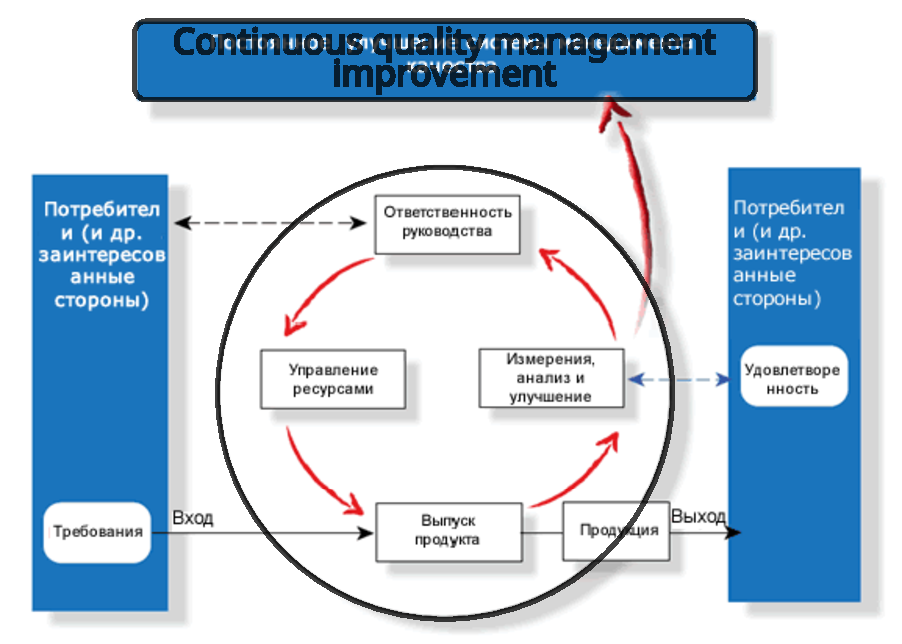
\includegraphics[width=0.6\linewidth]{qms-pics/iso9001.pdf}
  \caption{A general view on the ISO 9001/2015}
  \label{fig:iso9001}
\end{figure}


\section{Related work: programmatic SysML interpretation and code synthesis}

% From Ljubica
SysML is the dedicated system level UML-based notation proposed by the OMG. In research \cite{raslan} system design productivity is addressed as one of the main challenges. Some of the suggested approaches are increasing the level of abstraction and automation, as well as producing executable specifications. This research suggests that the automatic mapping of SysML, the system level UML based notations adopted by the OMG to SystemC, that was standardized by the IEEE, can raise the level of design abstraction in an automated environment and produce executable files.

In \cite{natale}, model driven development is used for the construction of complex embedded systems integrating software and firmware. A SysML system model is devised according to the platform-based design paradigm, in which a functional model of the system is paired to a model of the execution platform. Subsystems are refined as Simulink models or hand-coded in C++.

The SysML standard is attracting more attention of hardware designers as UML and SysML have been used to automatically generate an HDL code written in SystemC, Verilog and VHDL. In \cite{boute}, contrarily to the existing works, authors propose the new reverse engineering approach to generate SysML definition \textbf{bloc and internal bloc} diagrams from VHDL code. Code generation is done on the basis of a set of well-defined mapping rules between SysML and VHDL concepts.

UML profiles like SysML and MARTE have been a major research topic in electronic system design, but are mainly applied for specification and analysis in early design phases Research \cite{mish} addresses the problem of the High-Level Synthesis (HLS), i.e. physical implementation aspect of electronic systems which need diversity of design models and levels of abstraction.  To overcome the conflict between a higher degree of abstraction and necessary details for further synthesis, modular interfaces are introduced as object-oriented synthesizable technique. In \cite{mish},  SysML is used as an adequate modeling language for modular interfaces and C/C++/SystemC-based HLS. Authors extended SysML with annotations for synthesizable SystemC and high-level synthesis constraints and implemented a code generation scheme to achieve design flow automation. They used SysML editor Artisan Studio with industrial case study to demonstrate the applicability of SysML as a front-end for HLS design flows.

In \cite{tom16} UML/SysML is used to model avionics.  The implementation language is C\# with using libXML for XMI import and processing.  Generated objects represent each syntactic element (\texttt{struct}, \texttt{enum}, function, \emph{etc.}), which represents the target source code.  \textbf{... implemented only State Machine diagram}.

\cite{fab}

% Software interpreting ....


\section{Scheme of MDA implementation}
\label{sec:mda-impl-scheme}

\section{Conclusion}


\section{Acknowledgments}
\label{sec:acks}

The results are obtained with the partial support of The Council for grants of the President of Russian Federation, state support of leading scientific schools of the Russian Federation (NSH-8081.2016.9). The results obtained with the use of the network infrastructure of Telecommunication center of collective use "Integrated information-computational network of Irkutsk scientific-educational complex" (\url{http://net.icc.ru}).

\begin{thebibliography}{99}
%Related research
\bibitem{raslan} Waseem Raslan, Ahmed Sameh: Accelerating High-Level SysML and SystemC SoC Designs, URL:\url{https://www.design-reuse.com/articles/17562/high-level-sysml-systemc-soc-designs.html}
\bibitem{natale} Marco~Di~Natale,David~Perillo,Francesco~Chirico,Andrea~Sindico, Alberto~Sangiovanni-Vincentelli: “A Model-based approach for the synthesis of software to firmware adapters for use with automatically generated components”, Software \& Systems Modeling, February 2018,~Volume 17,~Issue~1,~pp.~11-–33
\bibitem{boute} Fateh Boutekkouk, Okba Fartas: Automatic generation of SysML diagrams from VHDL code, In Proceedings of the Symposium on Complex Systems and Intelligent Computing (CompSIC), Souk Ahras, Algeria, September 2015
\bibitem{mish} Fabian Mischkalla, Da He, Wolfgang Mueller, Florent Azcarate, Manuel Carballeda: A Retargetable SysML-based Front-End for High-Level Synthesis, In: Proceedings of 2nd Workshop on Model Based Engineering for Embedded Systems Design (M-BED) , Mrz. 2011
\bibitem{tom16}Tom Hauswald. Automatic Code Synthesis of UML/SysML State Machines for airborne Applications.  Bachelor Thesis. Hamburg Univeristy of Technology. August 15. 2016. 80~p.
\end{thebibliography}
\end{document}







%%% Local Variables:
%%% mode: latex
%%% TeX-master: "QMS-paper"
%%% End:
